% -*- mode:latex; mode:flyspell -*-
%%%%%%%%%%%%%%%%%%%%%%%%%%%%%%%%%%%%%%%%%%%%%%%%%%%%%%%%%%%%%%%%%%%%%%%%%%%%%%
\section{Correcting the relative tracker-calorimeter timing offset}

In an event that has a calorimeter cluster matched to a reconstructed track, the
cluster is included in the track fit as an additional hit. 
%
The straw hit reconstruction algorithm in the tracker and the waveform reconstruction 
algorithm in the calorimeter can add different timing offsets to the reconstructed straw hits
and calorimeter clusters respectively; these timing offsets need to be calibrated out.

The cluster is included in the track fit with a coordinate error $\sigma_{XY} = 15$ mm
and a timing error $\sigma_T = 0.5$ ns.
The distribution of the calorimeter cluster timing residuals for conversion electrons
using the default Kalman fit configuration is shown in Figure \ref{fig:track_cluster_dt}.a. 
The distribution of cluster timing residuals 
is centered at about -1.17 ns and has a width of about 0.34 ns, indicating a systematic timing offet.

To study the systematic offset and avoid biasing the fit, the errors assigned to the 
cluster were increased to $10^6$ ns and $10^6$ mm respectively,
the corresponding distribution in timing residuals is shown in Figure 
\ref{fig:track_cluster_dt}.b.
%
In this case, including the cluster in the track fit does not bias the result of the fit
and one can conclude that there is a systematic timing offset between the tracker
and the calorimeter of about 1.6 ns.
%
Figure \ref{fig:track_cluster_dt}.c corresponds to a fit configuration with
the increased errors and the cluster time corrected by 1.6 ns. So in a configuration
where the cluster in not biasing the fit results the applied correction zeroes
the timing offset.

The distribution of timing residuals with the cluster time corrected by 1.6 ns using
the default coordinate and timing errors, 0.5 ns and 15 mm respectively, 
assigned to the cluster shows a systematic shift of about 0.5-0.6 ns,
apparently introduced by the fitting procedure.
For now, we correct this additional cluster timing offset and use the default errors
assigned to the calorimeter cluster in the Kalman fit.
\footnote{
  Correction of the the global track-to-calorimeter timing offset has been introduced
  {\bf before} the tuning of the calorimeter timing resolution had been completed. 
  The global correction zeroing the offset of the timing residuals at that point 
  was 1.86 ns, so that was the value of the introduced timing offset constant.
  The observed timing offset value after the tuning is about 1.6 ns. 
  The resulting unaccounted for, systematic offset of about 0.25 ns is about x2 smaller
  than the offset introduced by the Kalman fitter.
}

% {\blue Not entirely clear what this paragraph is saying about the order of offsets
% and what the 1.86 ns offset is/came from, perhaps re-wording?}
% I moved the paragraph down the page, making it a  footnote.

It is also worth noting that the width of the distribution of the calorimeter cluster timing
residuals is approximately 50\% of the error assigned to the cluster.
The proportionality stays the same, about 50\%,  when the timing error assigned to the cluster
varies in the range [0.25 ns, 1 ns]. That is another indication of a uncompensated systematic effect
related to the use of the calorimeter cluster in the Kalman fit.

\begin{figure}[h]
  \hspace{-0.8in}
  \begin{tikzpicture}
    \node[anchor=south west,inner sep=0] at (0,0.) {
      % \node[shift={(0 cm,0.cm)},inner sep=0,rotate={90}] at (0,0) {}
      % \makebox[\textwidth][c] {
      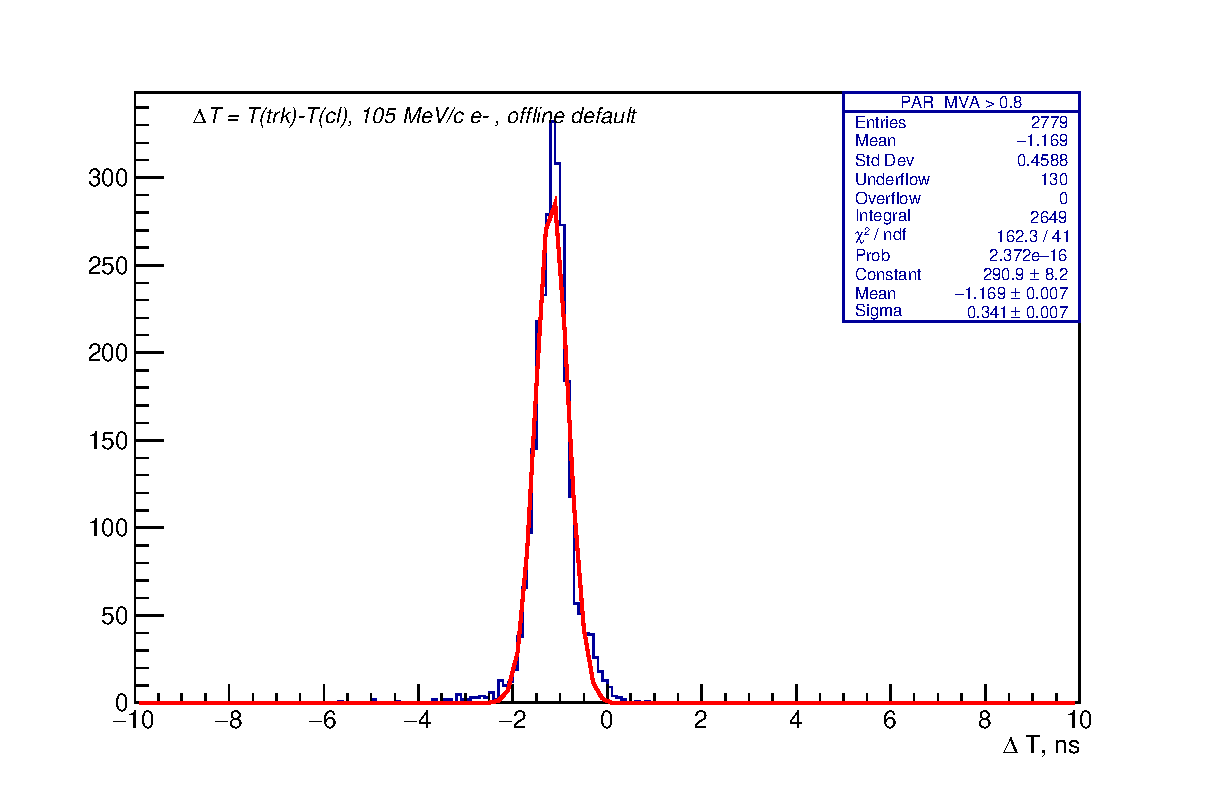
\includegraphics[width=0.64\textwidth]{figures/pdf/figure_00131_ele00s51b0_su2020_track_ana_trk_200_dt}
      % }
    };
    \node [text width=1cm, scale=0.8] at (3.,5) {(a)};
    \node[anchor=south west,inner sep=0] at (10.7,0.) {
      % \node[shift={(0 cm,0.cm)},inner sep=0,rotate={90}] at (0,0) {}
      % \makebox[\textwidth][c] {
      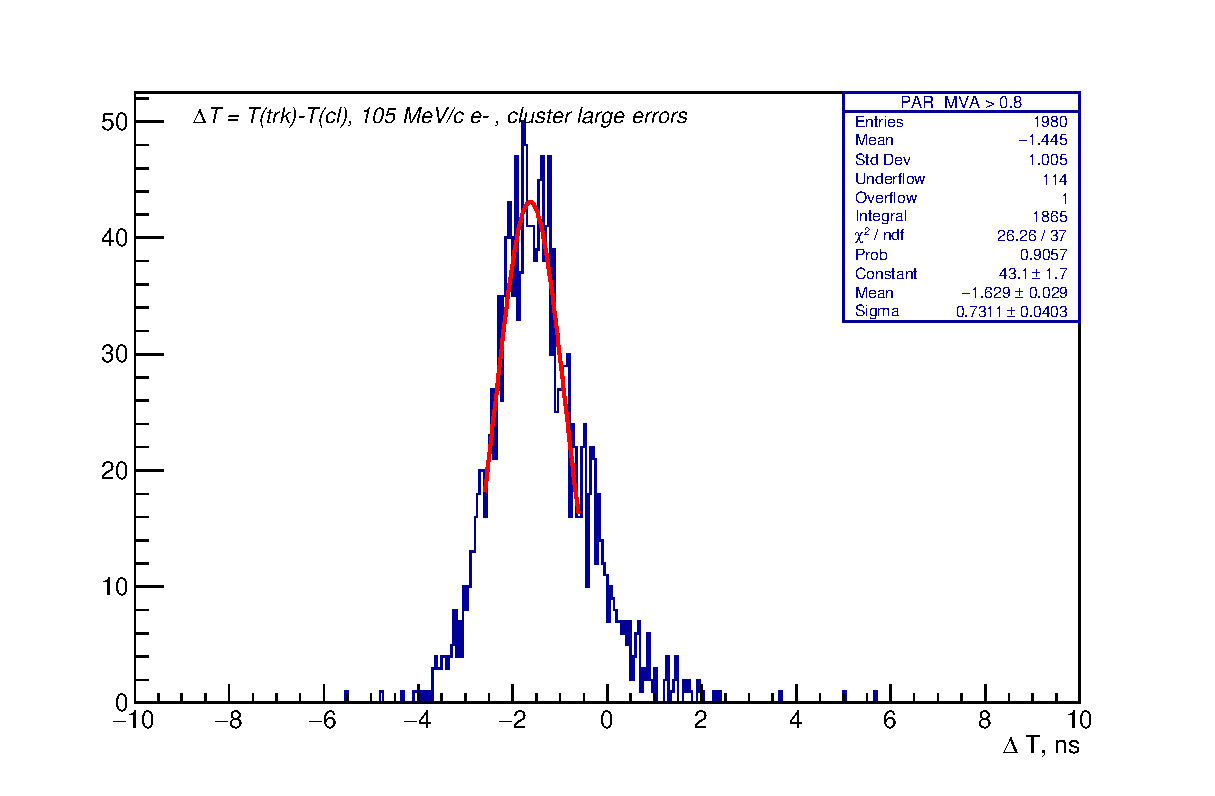
\includegraphics[width=0.64\textwidth]{figures/pdf/figure_00132_ele00s51b0_pid_emuana_trk_101_dt}
      % }
    };
    \node [text width=1cm, scale=0.8] at (13.7,5) {(b)};
    \node[anchor=south west,inner sep=0] at (0,-7.0) {
      % \node[shift={(0 cm,0.cm)},inner sep=0,rotate={90}] at (0,0) {}
      % \makebox[\textwidth][c] {
      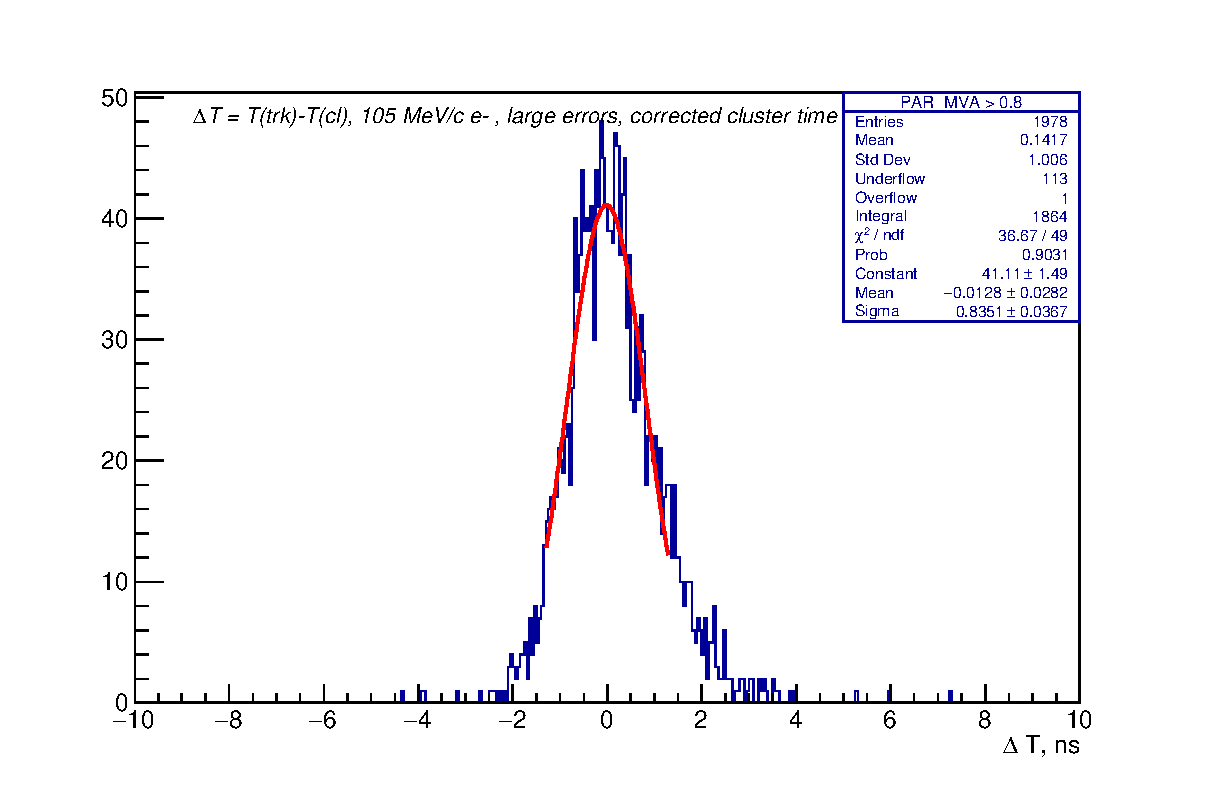
\includegraphics[width=0.64\textwidth]{figures/pdf/figure_00133_ele00s51b0_pid_emuana_trk_101_dt}
      % }
    };
    \node [text width=1cm, scale=0.8] at (3.,-2) {(c)};
    \node[anchor=south west,inner sep=0] at (10.7,-7.0) {
      % \node[shift={(0 cm,0.cm)},inner sep=0,rotate={90}] at (0,0) {}
      % \makebox[\textwidth][c] {
      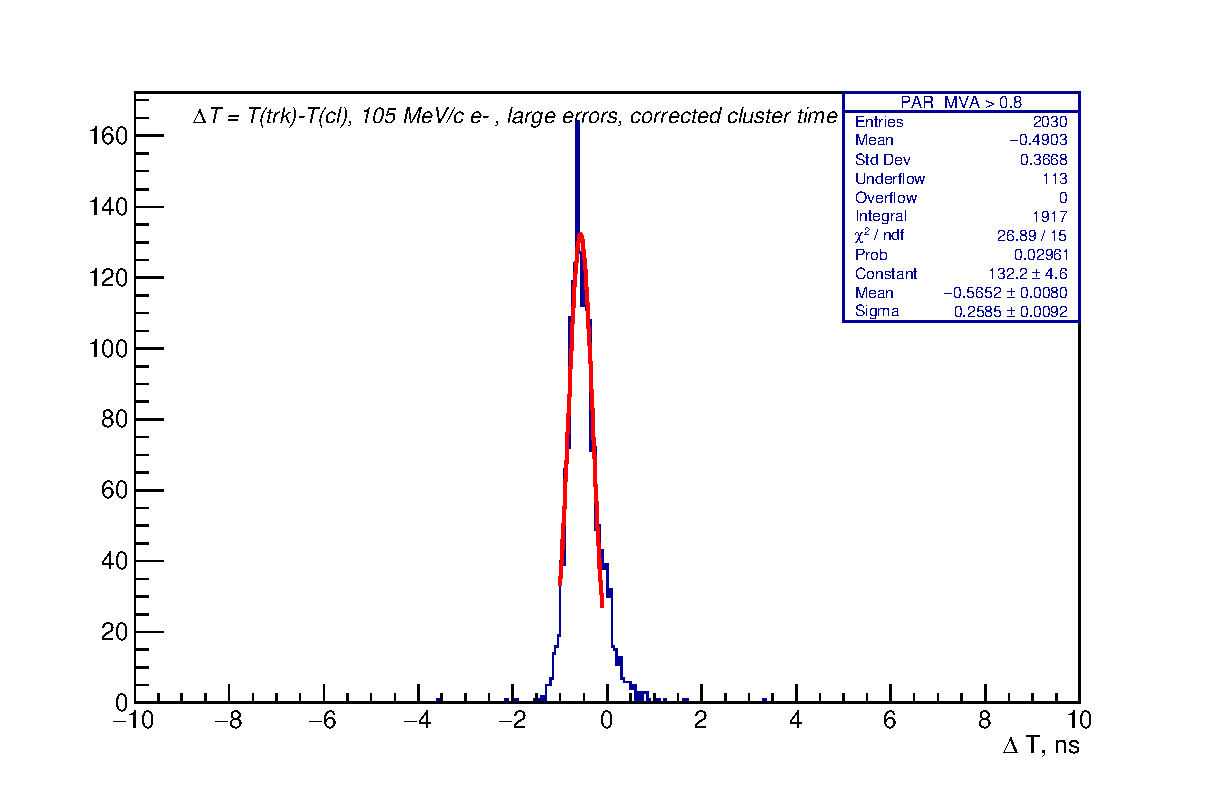
\includegraphics[width=0.64\textwidth]{figures/pdf/figure_00139_ele00s51b0_pid_emuana_trk_101_dt}
      % }
    };
    \node [text width=1cm, scale=0.8] at (13.7,-2) {(d)};
    % \node [text width=6cm, scale=0.8] at (4.5,6.4) {mu2e-18894 by Kevin Lynch and Jim Popp};
  \end{tikzpicture}
  % \captionof{figure} {
  \caption{
    \label{fig:track_cluster_dt}
    Track-cluster timing offsets and their correction: 
    (a) default offline configuration;
    (b) cluster assigned large errors in the fit; 
    (c) cluster timing corrected by 1.6 ns, still large errors;
    (d) cluster timing corrected by 1.6ns, default errors
  }
\end{figure}



%%% Local Variables:
%%% TeX-master: "mu2e-36375"
%%% End:
